% !TeX root = ../solution.tex

\hypertarget{he22.13}{%
\chapter{[HE22.13] Statues}\label{he22.13}}

\begin{marginfigure}
	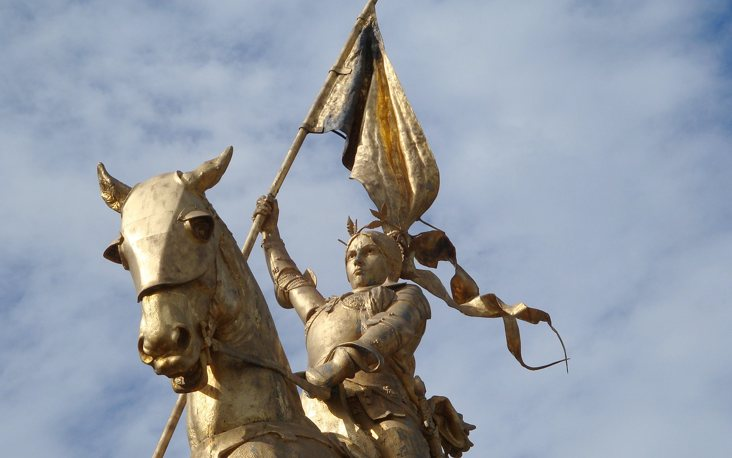
\includegraphics[width=49mm]{level4/challenge13.jpg}
\end{marginfigure}
\section{Intro}
Hope you like statues as much as I do!

I created a little tour in my favourite city for you:

\begin{enumerate}
\item    Richard I
\item     Peter Pan
\item     Albert
\item     James Cook
\end{enumerate}

I will not reveal my favourite statue, though. Find it yourself!

\subsection{{\NotoEmoji 🚩} Flag}

\begin{itemize}
	\item    it's not the one on the challenge image (Joan of Arc)!
	\item    name of the person represented by the statue
	\item    all lowercase, no spaces, no special chars
	\item    e.g. he2022{johnny} 
\end{itemize}

\section{Solution}\label{hv22.13solution}

The statues listed are all found in London, UK.  In Google Earth they are named
\begin{enumerate}
\item    Statue of Richard I of England
\item     Peter Pan Sculpture (by George Frampton)
\item     The Albert Memorial
\item     Captain James Cook Statue
\end{enumerate}

When the locations are plotted on a map, the lines from Richard I to Peter Pan
and from Albert to James Cook cross near the statue for the Duke of Wellington.
The statue depicts Achilles, so the flab becomes 
\verb+he2022{achilles}+.




